\documentclass[border=10pt]{standalone}
\usepackage[svgnames]{xcolor}
\usepackage{amsmath}
\usepackage{pgfplots}
\pgfplotsset{compat=newest}
\usepackage[sfdefault]{FiraSans}
\usepackage{FiraMono}
\renewcommand*\familydefault{\sfdefault}
\begin{document}
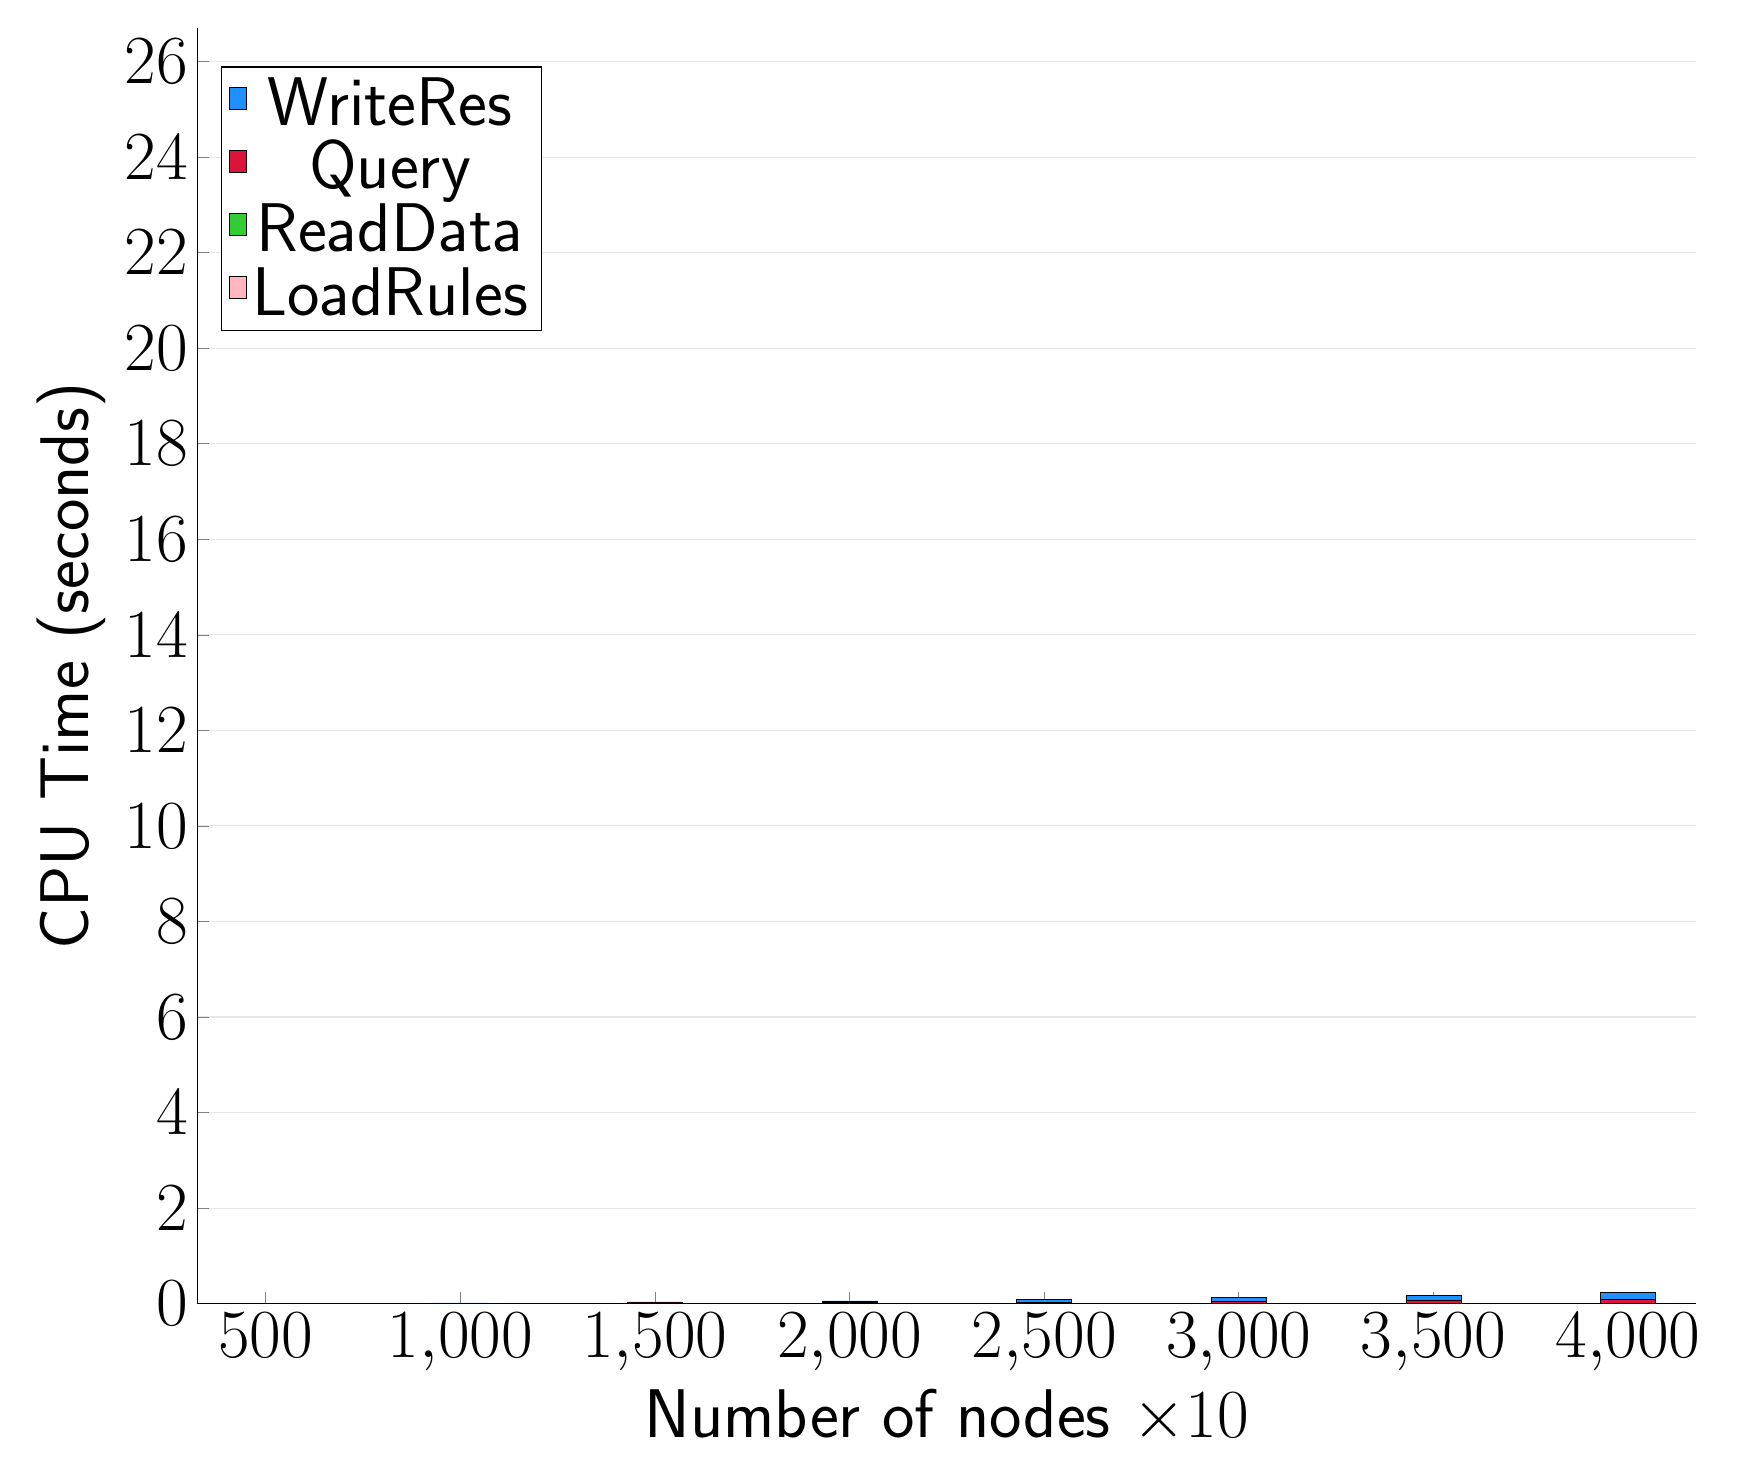
\begin{tikzpicture}
\begin{axis}[
   ybar stacked,
   width=1.7\textwidth,
   bar width=0.7cm,
   ymajorgrids, tick align=inside,
   major grid style={draw=gray!20},
   xtick=data,
   ymin=0, ymax=26.698890000000002,
   axis x line*=bottom,
   axis y line*=left,
   enlarge x limits=0.05,
   legend style={
       at={(0.23, 0.97)},
       anchor=north east,
       legend columns=1,
       font=\Huge,
   },
   ylabel={CPU Time (seconds)},
   xlabel={Number of nodes $\times 10$},
   label style={font=\Huge},
   tick label style={font=\Huge},
]
\addlegendimage{fill=DodgerBlue, draw=black, line width=0.2pt}
\addlegendentry{WriteRes}
\addlegendimage{fill=Crimson, draw=black, line width=0.2pt}
\addlegendentry{Query}
\addlegendimage{fill=LimeGreen, draw=black, line width=0.2pt}
\addlegendentry{ReadData}
\addlegendimage{fill=LightPink, draw=black, line width=0.2pt}
\addlegendentry{LoadRules}
\addplot +[fill=LightPink, draw=black, line width=0.2pt] coordinates {
(500, 0.0006163999999999998)
(1000, 0.0006118)
(1500, 0.0006055000000000004)
(2000, 0.0006146000000000004)
(2500, 0.0006238000000000001)
(3000, 0.0006349999999999996)
(3500, 0.0006086999999999993)
(4000, 0.0006159999999999997)
};
\addplot +[fill=LimeGreen, draw=black, line width=0.2pt] coordinates {
(500, 0.0005880000000000002)
(1000, 0.0010717)
(1500, 0.0015432)
(2000, 0.002051)
(2500, 0.0025302000000000002)
(3000, 0.0030497)
(3500, 0.0034939999999999997)
(4000, 0.0040036)
};
\addplot +[fill=Crimson, draw=black, line width=0.2pt] coordinates {
(500, 0.0011064)
(1000, 0.0045603)
(1500, 0.010622900000000001)
(2000, 0.0188502)
(2500, 0.0291761)
(3000, 0.0431721)
(3500, 0.057005099999999996)
(4000, 0.0783614)
};
\addplot +[fill=DodgerBlue, draw=black, line width=0.2pt] coordinates {
(500, 0.0022721000000000004)
(1000, 0.0093611)
(1500, 0.0209868)
(2000, 0.0367775)
(2500, 0.0568887)
(3000, 0.0822341)
(3500, 0.11212)
(4000, 0.14634699999999998)
};
\end{axis}
\end{tikzpicture}

\end{document}
